\documentclass[UTF8,12pt,a4paper]{article}
\usepackage{ctex}
\usepackage[top=2.54cm,bottom=2.54cm,left=2.8cm,right=2.8cm]{geometry}
\usepackage{graphicx}

%% 设置
\usepackage{ctex}  
\usepackage{amsmath, amsfonts, amssymb} % 数学公式相关宏包
\usepackage{color}      % color content
\usepackage{graphicx}   % 导入图片
\usepackage{subfigure}  % 并排子图
\usepackage{hyperref}
\usepackage{url}
%\usepackage{breakurl}	%网址换行
\usepackage{bm}         % 加粗部分公式,比如\bm{aaa}aaa
\usepackage{multirow}
\usepackage{booktabs}
\usepackage{longtable}  %长表格
\usepackage{supertabular}%跨页表格
\usepackage{changepage}
\usepackage{siunitx}%输入角度
\usepackage{appendix}
\newcommand{\mycomment}[1]{}%自定义注释。。

%修改字体,不会就去看刘海洋的书,不要自己瞎鼓捣
%ctex有的就直接用命令字体,可以不用这样调用\setCJKfamilyfont。当然renew后方便些
\usepackage{fontspec, xunicode, xltxtra}
\usepackage{xeCJK}		%中文字体
%%\setCJKfamilyfont{song}{SimSun}         %宋体 song,\songti
%\newcommand{\song}{\CJKfamily{song}}                        
%%\setCJKfamilyfont{fs}{FangSong_GB2312} %仿宋2312 fs,\fangsong
%\newcommand{\fs}{\CJKfamily{fs}}                            
%%\setCJKfamilyfont{yh}{Microsoft YaHei}  %微软雅黑 yh,\yahei 
%\newcommand{\yh}{\CJKfamily{yh}}  
%%\setCJKfamilyfont{hei}{SimHei}          %黑体  hei,\heiti 
%\newcommand{\hei}{\CJKfamily{hei}}    
%%\setCJKfamilyfont{hwxh}{STXihei}        %华文细黑  hwxh  
%\newcommand{\hwxh}{\CJKfamily{hwxh}}
%%\setCJKfamilyfont{asong}{Adobe Song Std}%Adobe 宋体  asong  
%\newcommand{\asong}{\CJKfamily{asong}}
%%\setCJKfamilyfont{ahei}{Adobe Heiti Std}%Adobe 黑体  ahei  
%\newcommand{\ahei}{\CJKfamily{ahei}}  
%%\setCJKfamilyfont{akai}{Adobe Kaiti Std}%Adobe 楷体  akai,\kaishu  
%\newcommand{\akai}{\CJKfamily{akai}}
%%\setCJKfamilyfont{hwsong}{STSong}                            %华文宋体  hwsong
%\newcommand{\hwsong}{\CJKfamily{hwsong}}
%%\setCJKfamilyfont{hwzs}{STZhongsong}                        %华文中宋  hwzs
%\newcommand{\hwzs}{\CJKfamily{hwzs}}
%%\setCJKfamilyfont{hwfs}{STFangsong}                            %华文仿宋  hwfs
%\newcommand{\hwfs}{\CJKfamily{hwfs}}
%%\setCJKfamilyfont{hwl}{STLiti}                                        %华文隶书  hwl
%\newcommand{\hwl}{\CJKfamily{hwl}}
%%\setCJKfamilyfont{hwxw}{STXinwei}                                %华文新魏  hwxw
%\newcommand{\hwxw}{\CJKfamily{hwxw}}
%%\setCJKfamilyfont{hwk}{STKaiti}                                    %华文楷体  hwk
%\newcommand{\hwk}{\CJKfamily{hwk}}
%%\setCJKfamilyfont{hwxk}{STXingkai}                            %华文行楷  hwxk
%\newcommand{\hwxk}{\CJKfamily{hwxk}}
%%\setCJKfamilyfont{hwcy}{STCaiyun}                                 %华文彩云 hwcy
%\newcommand{\hwcy}{\CJKfamily{hwcy}}
%%\setCJKfamilyfont{hwhp}{STHupo}                                 %华文琥珀   hwhp
%\newcommand{\hwhp}{\CJKfamily{hwhp}}
%%\setCJKfamilyfont{fzsong}{Simsun (Founder Extended)}     %方正宋体超大字符集   fzsong
%\newcommand{\fzsong}{\CJKfamily{fzsong}}
%%\setCJKfamilyfont{fzyao}{FZYaoTi}                                    %方正姚体  fzy
%\newcommand{\fzyao}{\CJKfamily{fzyao}}
%%\setCJKfamilyfont{fzshu}{FZShuTi}                                    %方正舒体 fzshu
%\newcommand{\fzshu}{\CJKfamily{fzshu}}


%\setCJKsansfont{\hei}%serif是有衬线字体sans serif无衬线字体。
%\setCJKmonofont{\fs}%mono字体
%\setCJKmainfont{Microsoft YaHei}  % 微软雅黑
%\setCJKmainfont{YouYuan}  % 幼圆,没有
%\setCJKmainfont{LiShu}  % 隶书
%\setCJKmainfont{NSimSun}  % 新宋体
%\setCJKmainfont{KaiTi}    % 楷体
\setCJKmainfont{SimSun}   % 宋体
%\setCJKmainfont{\hei}   % 黑体
%\setCJKmainfont{Segoe UI} %GitHub主题,不认中文

% -- 英文字体 --
\setmainfont{Times New Roman}
%\setmainfont{Consolas}
\setsansfont{Verdana}
%\setsansfont{DejaVu Sans}
%\setmonofont{Latin Modern Mono}

% 其他
%\usepackage{ccfonts} %公式使用concrete系列

% -- 字号设置 --
\newcommand{\chuhao}{\fontsize{42pt}{\baselineskip}\selectfont}
\newcommand{\xiaochu}{\fontsize{36pt}{\baselineskip}\selectfont}
\newcommand{\yihao}{\fontsize{28pt}{\baselineskip}\selectfont}
\newcommand{\erhao}{\fontsize{21pt}{\baselineskip}\selectfont}
\newcommand{\xiaoer}{\fontsize{18pt}{\baselineskip}\selectfont}
\newcommand{\sanhao}{\fontsize{15.75pt}{\baselineskip}\selectfont}
\newcommand{\sihao}{\fontsize{14pt}{\baselineskip}\selectfont}
\newcommand{\xiaosi}{\fontsize{12pt}{\baselineskip}\selectfont}     
\newcommand{\wuhao}{\fontsize{10.5pt}{\baselineskip}\selectfont}
\newcommand{\xiaowu}{\fontsize{9pt}{\baselineskip}\selectfont}
\newcommand{\liuhao}{\fontsize{7.875pt}{\baselineskip}\selectfont}

\usepackage{abstract}%修改摘要
\newcommand{\heiabstract}{\noindent\heiti 摘\hspace{1em}要:\songti}
\newcommand{\heikeyword}{\noindent\heiti 关键词:\songti}
\newtoks\myabstract%摘要
\newtoks\mykeywords%关键词
%\newcommand{\heirefname}{\heiti 参考文献:\song}
\renewcommand{\abstractname}{}%改摘要的格式
\newcommand{\upcite}[1]{$^{\mbox{\scriptsize \cite{#1}}}$}%参考文献的上标引用

%标题
\newtoks\subtitle
\makeatletter
\renewcommand*\maketitle{%
	\linespread{0.8}	
	\twocolumn[
	\begin{center}
		
		\xiaoer\heiti \@title\par 
		
		\begin{center} \renewcommand{\arraystretch}{1.5}
			\begin{tabular}{c}
				\xiaosi\fangsong	\@author \\
				\liuhao\songti		\the\subtitle \\
				\@date \\
			\end{tabular} \renewcommand{\arraystretch}{1}
		\end{center} 
		{\global\let\author\@empty}%
		{\global\let\date\@empty}%
	\end{center}%
	\linespread{1.0}
	\vspace{-5em}
	\begin{onecolabstract}
	\linespread{1.1}
	\xiaowu\heiabstract \the\myabstract

	\heikeyword \the\mykeywords
	\vspace{1.5em}
	\end{onecolabstract}]
	\setcounter{footnote}{0}%
}
\makeatother

%修改章节标题的字体,ctexart才能用
%用了ctexart,还使章节标题居中
\CTEXsetup[format={\xiaosi\heiti}]{section}
\CTEXsetup[format={\wuhao\heiti}]{subsection}
\CTEXsetup[format={\xiaowu\heiti}]{subsubsection}
%参考文献为小四黑体

%修改章节标题为中文
\usepackage{zhnumber}
%\renewcommand\thesection{\zhnum{section}}
%\renewcommand \thesubsection {\arabic{subsection}}
%\renewcommand \thesubsubsection {\arabic{subsection}.\arabic{subsubsection}}

%参考文献
%\usepackage{natbib}
%\usepackage[super]{gbt7714}%authoryear
%用选项代替\bibliographystyle{gbt7714-plain}unsrt


%\thispagestyle{empty}       %本页不显示页码
%\newpage                    %分页
%\tableofcontents\thispagestyle{empty}
%\setcounter{page}{1}        %从下面开始编页,页脚格式为导言部分设置的格式

\usepackage{enumitem}%修改列表环境
\setenumerate[1]{itemsep=0pt,partopsep=0pt,parsep=\parskip,topsep=5pt}
\setitemize[1]{itemsep=0pt,partopsep=0pt,parsep=\parskip,topsep=5pt}
\setdescription{itemsep=0pt,partopsep=0pt,parsep=\parskip,topsep=5pt}

%自定义微分号
\newcommand{\di}[1]{\mathrm{d}#1}
\newcommand{\p}[2]{\frac{\partial #1}{\partial #2}}
\newcommand{\pp}[2]{\frac{\partial ^2 #1}{\partial #2 ^2}}
\newcommand{\dy}[2]{\frac{\di{#1}}{\di{#2}}}
\newcommand{\ddy}[2]{\frac{\mathrm{d} ^2 #1}{\mathrm{d} #2 ^2}}



% 定义页眉和页脚
\usepackage{fancyhdr}
%\fancypagestyle{plain}
%\pagestyle{fancyplain}

%彩色文本框
\usepackage{tcolorbox}
\tcbuselibrary{skins, breakable, theorems}
\usepackage{colortbl}
\tcbset{colframe = blue!50!black, colback = white,
	colupper = red!50!black, fonttitle = \bfseries,
	nobeforeafter, center title}

%更改脚注格式
\renewcommand{\thefootnote}{\color{red}\arabic{footnote}}

%插入代码
\usepackage{listings}
\lstset{%自己定制的MATLAB格式,用mcode字体为啥不太好
	backgroundcolor=\color{red!5!green!5!blue!0},%代码块背景色为浅灰色
	rulesepcolor= \color{gray}, %代码块边框颜色
	breaklines=true,  %代码过长则换行
	numbers=left, %设置行号位置
	numberstyle=\scriptsize, %设置行号大小
	basicstyle=\sffamily,% 基本代码风格
	keywordstyle=\color{blue}, %设置关键字颜色\bfseries
	commentstyle=\rmfamily\color[cmyk]{1,0,1,0}, %设置注释颜色
	stringstyle=\ttfamily\color{red!60!green!40!blue!80},
	frame=shadowbox,%用方框框住代码块
	%frame=singl
	escapeinside=``, %逃逸字e, %设置边框格式符(1左面的键),用于显示中文
	extendedchars=false, %解决代码跨页时,章节标题,页眉等汉字不显示的问题
	xleftmargin=2em,xrightmargin=2em, aboveskip=1em, %设置边距
	tabsize=4, %设置tab空格数
	showspaces=false, %不显示空格
	showstringspaces=false,
	captionpos=t,% 这段代码的名字所呈现的位置,t指的是top上面
	columns=fullflexible
}
%\usepackage[framed,numbered,useliterate]{mcode}
%basicstyle= \sffamily,% 基本代码风格
%stringstyle= \ttfamily,
%commentstyle=\rmfamily\itshape,%注释的风格,斜体

%罗马数字
\newcommand{\RNum}[1]{\uppercase\expandafter{\romannumeral #1\relax}}

%写化学式
\usepackage[version=4]{mhchem}
\usepackage{setspace}%调行距
%\setstretch{1.25}
\linespread{1.25}
\graphicspath{{pics/}}





%% 信息
\title{西安交通大学课程作业\LaTeX 模板}%长标题请手动换行
\author{高旭帆}  %高旭帆\\ \xiaowu (西安交通大学生命学院,化生试验班,西安\hspace{0.5em}710049)
\stuId{2186113574}
\class{化生81}
\school{生命学院}
\course{马克思主义基本原理}
\date{\today}
\subtitle{这是副标题}
\myabstract{摘要内容一般包括:从事这项研究工作的目的和意义;完成的工作 (作者独立进行的研究工作及相应结果的概括性叙述);获得的主要结论 (这是摘要的中心内容)。论文摘要应突出论文的创新点。
摘要中一般不用图、表、化学结构式、非公知公用的符号和术语。
如果论文的主体工作得到了有关基金资助,应在摘要第一页的页脚处标注:本研究得到某某基金 (编号:) 资助。}
\mykeywords{西安交通大学;课程作业论文;\LaTeX{} 模板}

\begin{document}
% 设置标题
%标题页格式
\definecolor{MyLightBlue}{rgb}{0.8,1,1}

\let\origbaselineskip\baselineskip % 标题内部行距

% 无副标题的单双栏好了

\makeatletter

\begin{titlepage}
%	\pagecolor{MyLightBlue} % 背景颜色
	\begin{center}
		\begin{figure*}[!ht]\vspace{2em}
			\centering
			
\includegraphics[width=0.5\textwidth]{xjtu}
		\end{figure*}

		\vspace{1em}	
		\heiti\erhao  课程作业 
		
		\vspace{2.3em}	
		\vspace{1em}		

		% 居中标题
		\begin{textblock*}{\textwidth}(1.15in+\hoffset,10cm) % {block width} (coords) 
			\centering
			\setlength{\baselineskip}{1.4\origbaselineskip} % 内部行距
			\heiti\chuhao \thetitle 
			
			
			\vspace{0.5em}
			\ifsubtitleexist
			\songti\yihao \the\subtitle
			\else
			\hrule 
			\vspace{0.5em}
			\pgfornamenthan[scale=0.4]{60}
%			\pgfornamenthan[scale=0.15]{58}
			\fi
		\end{textblock*}
		
		
		\vspace{13em}
		
		{\sanhao\yh\renewcommand{\arraystretch}{1.5}\renewcommand{\baselinestretch}{1.2}
		\begin{tabular}{c}
			姓名:\@author \\
			学号:\the\stuId \\
			班级:\the\class \\
			学院:\the\school \\
			\ifcsname @extrainfo\endcsname \@extrainfo\\ \fi
%			课程:\the\course\\ % 将来可做个选项,不仅可选,还要调整位置
			\@date \\
		\end{tabular}} 
			
		\renewcommand{\arraystretch}{1}
		{\global\let\author\@empty}%
		{\global\let\date\@empty}%
		\setcounter{footnote}{0}%
	\end{center}
	\begin{tikzpicture}[remember picture, overlay]
		\begin{pgfonlayer}{background}
		\node at ($(current page.south) +(0in,2.5in)$) {%
			
\includegraphics[width=0.8\textwidth]{cover.png}};
		\end{pgfonlayer}
	\end{tikzpicture}
	\clearpage{\pagestyle{empty}\cleardoublepage}
\end{titlepage}
\makeatother

\newpage

\ifabstractexist
	\begin{center}
		\sanhao\selectfont\song
		摘\hspace{2em}要
	\end{center}
	\vspace{\baselineskip}
	\setcounter{page}{1}
	%\pagenumbering{Roman}
	\xiaosi
	
	\heiabstract \the\myabstract
	
	\vspace{\baselineskip}
	\heikeyword \the\mykeywords
	
	\vspace{\baselineskip}
	
	\begin{tikzpicture}[remember picture, overlay]
	\begin{pgfonlayer}{background}
	\node at ($(current page.south) +(0in,2.5in)$) {%
		
\includegraphics[width=0.8\textwidth]{cover.png}};
	\end{pgfonlayer}
	\end{tikzpicture}
	
	\setcounter{footnote}{0}
	\setcounter{page}{0}
	\clearpage
\fi
%单独页标题
\begin{center}
	\sanhao\selectfont\song
	摘\hspace{2em}要
\end{center}
\vspace{\baselineskip}
\setcounter{page}{1}
%\pagenumbering{Roman}
\xiaosi

\heiabstract \the\myabstract

\vspace{\baselineskip}
\heikeyword \the\mykeywords

\vspace{\baselineskip}
%\heitypeofthesis 应用基础

\setcounter{footnote}{0}
\setcounter{page}{0}
\clearpage%单独页摘要	
%\makeatletter
\renewcommand*\maketitle{%
	\linespread{0.8}	
	\begin{center}
		{\xiaoer\heiti \@title}
		
		\begin{center} \renewcommand{\arraystretch}{1.5}
			\begin{tabular}{c}
				\sihao \@author \\
				%\wuhao\@date \\
			\end{tabular} \renewcommand{\arraystretch}{1}
		\end{center} 
		{\global\let\author\@empty}%
		{\global\let\date\@empty}%
	\end{center}%
	\linespread{1.0}
	\vspace{-3.5em}
	\begin{abstract}
		\linespread{1.1}
		\wuhao\heiti 摘\hspace{0.8em}要:\kaishu \the\myabstract
		
		\wuhao\heiti 关键词:\kaishu \the\mykeywords
		\vspace{1.5em}
	\end{abstract}
	\setcounter{footnote}{0}
	\setcounter{page}{0}
}
\makeatother


\maketitle%普通标题
%正常标题+摘要
%\makeatletter
\renewcommand*\maketitle{%
	\linespread{0.8}	
	\twocolumn[
	\begin{center}
		{\xiaoer\heiti \@title}
		
		\begin{center} \renewcommand{\arraystretch}{1.5}
			\begin{tabular}{c}
				\sihao \@author \\
				%\wuhao\@date \\
			\end{tabular} \renewcommand{\arraystretch}{1}
		\end{center} 
		{\global\let\author\@empty}%
		{\global\let\date\@empty}%
	\end{center}%
	\linespread{1.0}
	\vspace{-3.5em}
	\begin{onecolabstract}
		\linespread{1.1}
		\wuhao\heiti 摘\hspace{0.8em}要:\kaishu \the\myabstract
		
		\wuhao\heiti 关键词:\kaishu \the\mykeywords
		\vspace{1.5em}
	\end{onecolabstract}]
	\setcounter{footnote}{0}
	\setcounter{page}{0}
}
\makeatother


\maketitle%普通标题%双栏版,可能要调列表行距
%1,3、2,3不要混用


\section{文字}
\LaTeX 是一个功能强大的特别适合排版科技文献和书籍的格式化排版程序。它是由著名计算机专家和数学家斯坦福大学D.E.Knuth教授研制的。20世纪60年代,knuth准备出系列专著《计算机程序设计技巧》(The Arts of Computer Programming),前三册已经出版,当他正在撰写第四册时,出版社拿来第二册的第二版给他过目,结果令他大失所望,因为当时出版社的印刷技术没有使他的书稿更好看,反而变糟了,尤其是在数学公式和字体上面的缺陷更令他无法接受。于是他就打算自己写一个既能供科学家编排手稿又符合出版社印刷要求的高质量的计算机排版系统。这就是TeX排版系统的由来。

TeX系统是由Pascal语言编写的,程序的源代码也是公开的。它包含300条基本命令和600条扩展命令,几乎可以排版任何格式的文献,如一般文章、报告、书刊和诗集等,对数学公式的排版也被公认是最好的。TeX系统的优点之一是它还支持命令宏,这使得使用TeX成为一种乐趣,用户可以自己编写宏包来定义更多、更方便的新命令,这也是TeX能得以迅速发展的原因。而且TeX是一个可移植性系统,可以运行于所有类型的计算机(如苹果机、IBM PC机及大型工作站)和各种操作系统(如DOS、Windows、Unix等),它的排版结果dvi文件于输出设备无关,可以在不同的操作系统上显示和打印。TeX源文件是ASCII码文件,可以方便地在网络上传播。目前,大多数学术部分和校园网上都安装有TeX系统。国际上许多出版机构也采用TeX系统来排版书刊,不少出版社还要求作者提供手稿的TeX源文件。

虽然TeX的功能非常强大,用它可以排版任何式样的文稿,但普通用户要灵活掌握TeX的900条初始命令还是有困难的。因而,TeX公开几年后,利用 TeX的宏定义功能开发的宏库AMSTeX和LaTeX就产生了。AMSTeX是Michael Spaivak受美国数学会(AMS)的委托编写的,重要用于AMS和其他分支机构出版的大量书籍、期刊和评论。AMSTeX含有一个宏包(Style file),供作者用来方便的准备稿件。用AMSTeX可以方便地排印出非常复杂的数学公式和AMS制定的全部数学符号。

LaTeX是由美国计算机学家Leslie Lamport于1985年开发成功的。尽管在排版数学公式和数学符号方便LaTeX不如AMSTeX,但LaTeX提供了大量易于学习和使用的命令,如非常有用的交叉引用命令(cross-referencing commands),这是AMSTeX所不具备的。因而LaTeX有更广泛的用途,特别是在排版信件、书刊、诗集等方面更优于AMSTeX。TeX的命令好比是建筑所使用的各种各样的材料,优秀的建筑师用它能建造出各种美丽的建筑;LaTeX的命令好比是已经建筑好的各种各样的房间和家具,用户只需选择适合自己的房间和家具就能得到满意的住所,而且这种房间和家具之多几乎无须用户自己动手建造。为了使用户既能使用LaTeX提供的大量命令,又能排版出优美的数学公式和数学符号,美国数学会又开发了AMSTeX。

TeX的使用相对于word要麻烦很多,但是其优势势非常明显的,就举几个吧。word中数学公式是以图片形式保存的,一旦公式和图片多的话则很容易死机,偶在竞赛中则吃过大亏,在全国赛和国际赛中都发生过这些情况,辛辛苦苦写了很多,但是全部没了,那时真是欲哭无泪啊。现在是学乖了,用word写论文时时常按ctrl+s。并且不同版本不兼容,xp版本到2000版本就出现很严重的不兼容问题。而LaTeX则不会出现这种情况。用word写论文时可以发现当公式或数学符号在某行中时则行距撑的艽罅耍帜芽矗琇aTeX则不会出现这种问题。说到公式和数学符号则可很明显的感觉到word和LaTeX 的不同了,爱美之心人皆有之,学数学的很大程度也是因为被数学的美所深深的吸引而迷恋数学。而LaTeX排版出来的数学公式则比word要漂亮的多了。此外在写论文的时候对参考文献十分头痛,而LaTeX则在这个方面不要比word显的太强悍啊。

介绍了这么多LaTeX并不是说明LaTeX比word怎么怎么牛,每个事物存在就有它存在的的价值,word在很多地方有比LaTeX很明显的优势。只不过在数学论文这个方面LaTeX要比word强太多了,故而介绍这么多,推荐使用LaTeX写数学论文。

\vspace{0.5em}\noindent%必须有
\begin{tcolorbox}
	这是一个tcolorbox。
	公司表示:“项目在来承传统工艺的基础上,集节能减排、清洁生产、资源循环利用:所化融合为一体,全面实施了自动化、数字化、智能化全面升级改造。开级改造后,企业产品成本更低,品质更高,将更具市场竞争力,一期工程竣工落成,预示着秦洋长生酒业转型升级成功。”
\end{tcolorbox}

\section{实验原理}
\subsection{1}
\subsection{2}

\section{实验仪器与试剂}
\subsection{仪器}
\subsection{试剂}

\section{实验步骤}
\begin{enumerate}
	\item 找到激光器电源模块,打开开关,出现激光。
	\item 调节激光,保证功率在200mW以上,波长在532.8nm左右。
	\item 第一个空间光调制器选择HG模式,输入合适的参数,观察光栅的样式,打开接收高阶高斯光的CCD相机,观察高阶高斯光。
	\item 调节第一个空间光调制器的位置,进行微调,使得在CCD上观察到的高阶高斯光能够完全显示。
	\item 转化成LG高斯模式,观察CCD上的图案。
	\item 调节双柱透镜,保证其焦距是两个透镜间距的一半,高斯光通过之后转换高斯模式,通过CCD观察。
	\item 调节第二个空间光调制器,选择分束模式。
	\item 打开显微镜控制模块,产生显微镜照明灯光。
	\item 打开最后一个CCD,调出微粒自旋的效果。
	\item 让最后一个CCD上出现拉盖尔高阶高斯光,观察微粒自旋和公转的效果。
\end{enumerate}

\section{思考题}
\begin{enumerate}
	\item sf
	\item df
\end{enumerate}

\section{例子}
\subsection{实验题目}
某医院用光电比色计检验尿汞时,得尿汞含量与消光系数读数的结果如下表:
\begin{table}[!h]
	\centering
	%\caption{Add caption}
	\begin{tabular}{cccccc}
		\toprule
		尿汞含量X & 2     & 4     & 6     & 8     & 10 \\
		\midrule
		消光系数Y & 64    & 138   & 205   & 285   & 360 \\
		\bottomrule
	\end{tabular}%
	\label{tab:exercise8_3}%
\end{table}%

\begin{enumerate}
	\item 画出散点图;
	\item 试求回归系数及方差的估计值;
	\item 对回归方程作显著性检验;
	\item 求当$x_0=12$时,因变量$Y$的观测值$y_0$的预测值及置信度为$0.95$的置信区间。
\end{enumerate}

\subsection{所建立的数学模型、编程思想}
该题应利用[b,bint,r,rint,stats]=regress(Y,X)函数来求解回归系数及其各项参数,从而通过stats(3)验证其显著性,stats((4)即为其方差,而后根据所求参数构造函数并绘图。将$x_0$代入回归方程求解预测值,利用
\begin{equation*}
\scriptstyle\left(y_f-t_{\alpha/2}\cdot\sqrt{\left(1+\dfrac{1}{n}+\dfrac{{\left(x_f-\overline{x}\right)}^2}{\sum_{i=1}^{n}}{{(x_i-\overline{x})}^2}\right)\hat{\sigma_u}^2}\ ,\ y_f+t_{\alpha/2}\cdot\sqrt{\left(1+\dfrac{1}{n}+\dfrac{{\left(x_f-\overline{x}\right)}^2}{\sum_{i=1}^{n}}{{(x_i-\overline{x})}^2}\right)\hat{\sigma_u}^2}\right)
\end{equation*}
求解置信区间。

\subsection{插入图片}

\begin{figure}[!h]
	\centering
	\begin{minipage}[c]{0.45\textwidth}
		\centering
		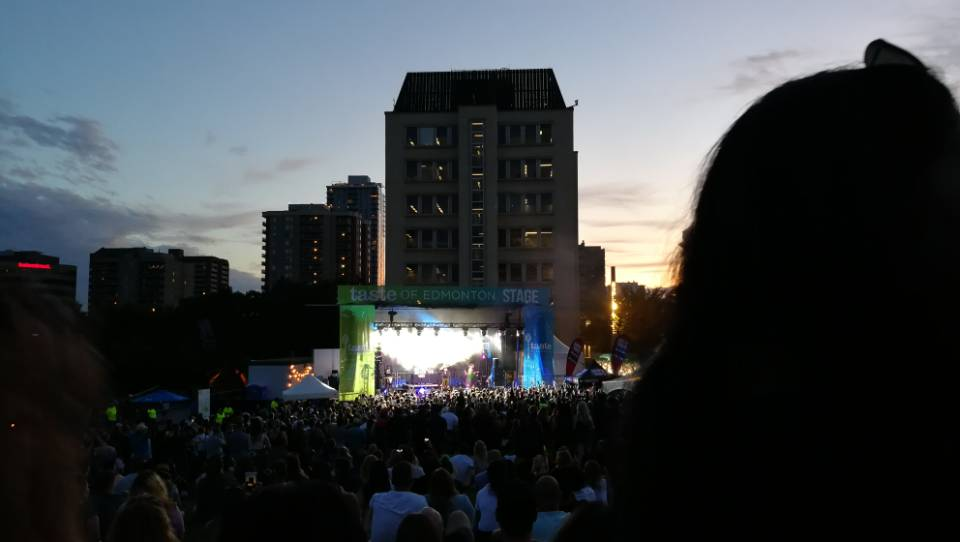
\includegraphics[width=\linewidth, height=0.4\textheight]{city}
	\end{minipage}
	\quad
	\begin{minipage}[c]{0.45\textwidth}
		\centering
		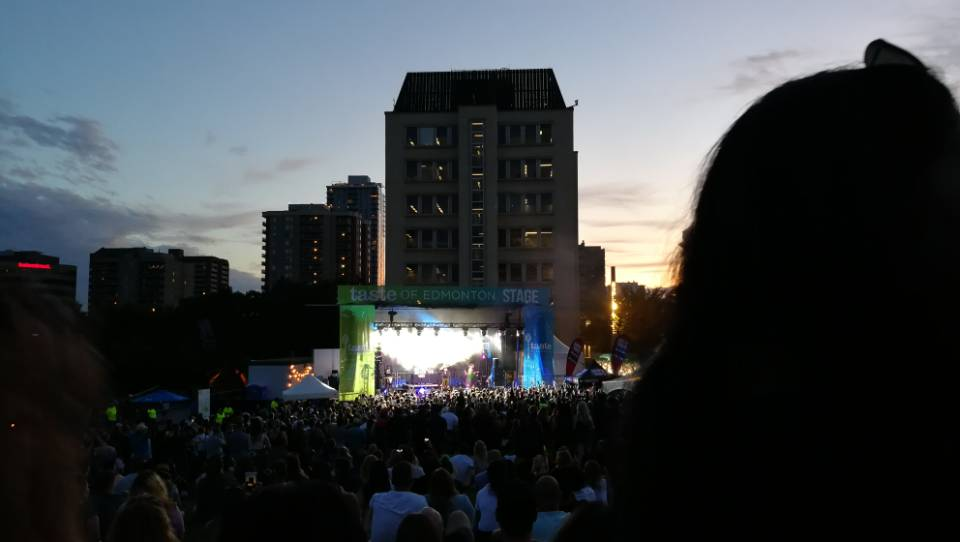
\includegraphics[width=\linewidth, height=0.4\textheight]{city}
	\end{minipage}
	\caption{固定长宽}
\end{figure}

\begin{figure}[htbp]
	\centering
	\setlength{\subfigcapskip}{6pt}
	\subfigure[夜幕降临]{
		\begin{minipage}[t]{0.42\linewidth}
			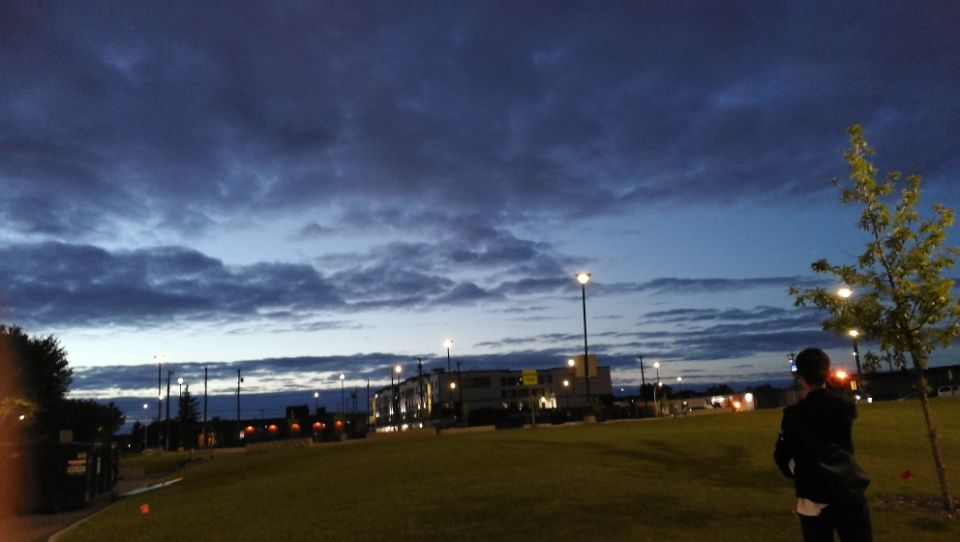
\includegraphics[width=\textwidth]{nightfall.jpg}
	\end{minipage}}
	\quad
	\subfigure[北萨斯喀彻温河]{
		\begin{minipage}[t]{0.42\linewidth}
			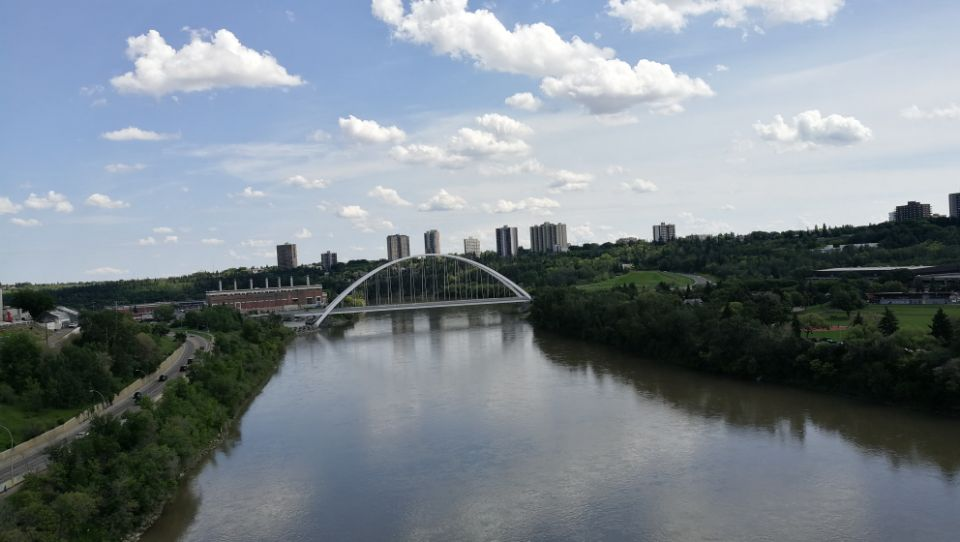
\includegraphics[width=\textwidth]{NorthSaskatchewanRiver.jpg}
	\end{minipage}}
	
	\subfigure[鸭子湖公园]{
		\begin{minipage}[t]{0.42\linewidth}
			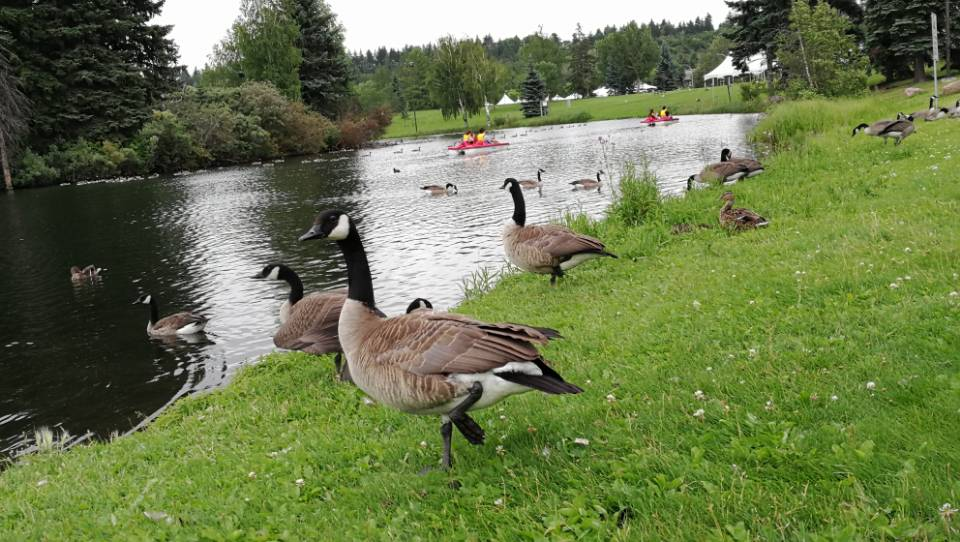
\includegraphics[width=\textwidth]{HawrelakPark.jpg}
	\end{minipage}}
	\quad
	\subfigure[“体验埃德蒙顿”美食音乐节]{
		\begin{minipage}[t]{0.42\linewidth}
			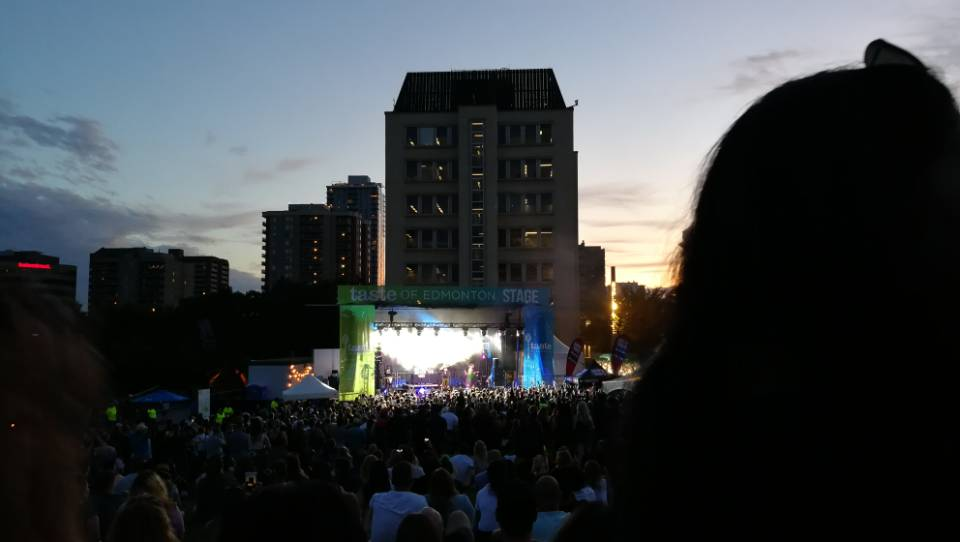
\includegraphics[width=\textwidth]{city.jpg}
	\end{minipage}}
	\caption{城市风景}
\end{figure}


举个例子,你总是想预测给定四个单词(上图编号1所示)后的下一个单词,注意这里的4是算法的超参数。这就是如何适应很长或者很短的句子,方法就是总是只看前4个单词,所以说我只用这4个单词(上图编号2所示)而不去看这几个词(上图编号3所示)。

\begin{appendices}
在正文中添加附录
\end{appendices}

\subsection{结果分析及说明}
\begin{enumerate}
	\item 画出散点图如图所示;
	\item 回归系数为$a=-11.30$,$b=36.95$,方差估计值为$12.3667$;
	\item 由于regress函数所用F检验$p=0$,且$p<0.01$时可认为回归方程高度显著,故可认为该回归方程是高度显著的;
	\item $y_0$的预测值为$432.10$,置信度为$0.95$的置信区间为$[415.8822,448.3178]$。
\end{enumerate}

\subsection{实验总结与体会}
通过对回归分析及MATLAB软件在概率统计中的应用两章的自学,在查找资料和咨询老师同学的过程中,我对MATLAB软件在概率论这门课程中的应用有了更加深入的了解,掌握了一定的技能,并且更直观的看到了概率统计的意义,在此过程中也对许多概念有了更加深入的了解和感悟,十分有益于概率论课程的学习。



\section{结束语}
欢迎大家为我东拼西凑的\LaTeX 模板提出建议!


%参考文献
\begin{thebibliography}{2}
	\bibitem{1} hahahaha
	\bibitem{2} lalalala
\end{thebibliography}
%使用bib文件
%\bibliographystyle{./template/gbt7714-unsrt}
%\bibliography{reference}



\appendix
%\renewcommand{\appendixname}{Appendix~\Alph{section}}
\addappheadtotoc%添加进目录

\newpage

\begin{center}
	\Huge\bfseries\heiti 附录 % Appendix
\end{center}

\section{code}

This is some Matlab code
\subsection{程序}
\begin{lstlisting}[language={Matlab},morekeywords={regress}]
clear;
x=[2,4,6,8,10];
y=[64,138,205,285,360];
n=length(x);
X=[ones(length(y),1),x&apos;];
Y=y&apos;
[b,bint,r,rint,stats]=regress(Y,X);
%b为回归系数,bint为回归系数的区间估计
%r为残差,rint为残差置信区间
%stats对应相关系数R²,F值,与F对应的概率p,误差方差
y_hat=b(1)+b(2)*x;
plot(x,Y,&apos;k*&apos;,x,y_hat,&apos;r&apos;);%绘图
%预测x0=12时y0的值
xf=12;
yf=b(1)+b(2)*xf;
\end{lstlisting}


%\lstinputlisting[language=python]{./code/TFIDF.py}


\end{document}